\documentclass[t,pdf]{beamer}
\mode<presentation>{}


\usecolortheme[RGB={196, 30, 58}]{structure}

\usepackage{color}
\usepackage{animate}
\usepackage{tikz}
\usetikzlibrary{shadings,shadows}
\usetikzlibrary{shapes, arrows}
\usetikzlibrary{decorations.pathreplacing,angles,quotes}
\usetikzlibrary{calc}
\usetikzlibrary{positioning}
\usepackage{pgfplots}
\usepackage{booktabs}
\usepackage{alltt}
\usepackage{bussproofs}

\newenvironment{ccode}{\begin{alltt}\footnotesize}{\end{alltt}}

\usepackage{booktabs,colortbl}

\usepackage{hyperref}
%% Colored hyperlink 
\newcommand{\cref}[2]{\href{#1}{\color{blue}#2}}
%% Colored hyperlink showing link in TT font
% \newcommand{\chref}[1]{\href{#1}{\small\tt \color{blue}#1}}
\newcommand{\hcref}[1]{\cref{#1}{\small\tt #1}}


\newcommand{\ground}{blue}

\newcommand{\ft}[1]{\frametitle{#1}}
\newcommand{\ig}[2]{\includegraphics[#1]{#2}}

\definecolor{xred}{rgb}{0.77, 0.12, 0.23}
\definecolor{xgreen}{rgb}{0.3, 0.6, 0}
\definecolor{xblue}{rgb}{0., 0.25, 1}
\tikzstyle{grayfill} = [fill=fillcolor!70, draw=drawcolor, thick]
\tikzstyle{whitefill} = [fill=white, draw=drawcolor, thick] 
\definecolor{fillcolor}{rgb}{0.5, 0.5, 0.5} 
\definecolor{drawcolor}{rgb}{0, 0, 0} 

\newcommand{\hdomino}[2]{\draw [draw=black, fill=black, rounded corners=2pt] (#1+0.1,#2+0.1) rectangle (#1+1.9,#2+0.9);}
\newcommand{\vdomino}[2]{\draw [draw=black, fill=black, rounded corners=2pt] (#1+0.1,#2+0.1) rectangle (#1+0.9,#2+1.9);}

\newcommand{\hdomina}[2]{\draw [draw=black, fill=black, rounded corners=2pt] (#1+0.1,#2+0.1) rectangle (#1+1.9,#2+0.9);
                                              \draw [very thick, draw=xgreen] (#1,#2) rectangle (#1+2,#2+1);
                                              \draw [very thick, draw=structure] (#1+1,#2) -- (#1+1,#2+1);}
\newcommand{\hdominah}[2]{\draw [draw=black, fill=black, rounded corners=2pt] (#1+0.1,#2+0.1) rectangle (#1+1.9,#2+0.9);
%                                              \draw [very thick, draw=xgreen] (#1,#2) rectangle (#1+2,#2+1);
                                              \draw [very thick, draw=structure] (#1+1,#2) -- (#1+1,#2+1);}
\newcommand{\vdomina}[2]{\draw [draw=black, fill=black, rounded corners=2pt] (#1+0.1,#2+0.1) rectangle (#1+0.9,#2+1.9);
                                              \draw [very thick, draw=xgreen] (#1,#2) rectangle (#1+1,#2+2);
                                              \draw [very thick, draw=structure] (#1,#2+1) -- (#1+1,#2+1);}

\newcommand\setrow[9]{
  \setcounter{col}{1}
  \foreach \n in {#1, #2, #3, #4, #5, #6, #7, #8, #9} {
    \edef\x{\value{col} - 0.5}
    \edef\y{9.5 - \value{row}}
    \node[anchor=center] at (\x, \y) {\n};
    \stepcounter{col}
  }
  \stepcounter{row}
}

\font\dominos=domino
\def\die#1{{\dominos#1}}

\newcommand\PlaceDot[2]{\fill[white] ([shift={(#1,#2)}]0,0) circle [radius=0.08];}

\newcommand\domino[1]{
{
\ifcase#1\relax
\or \PlaceDot{0}{0}
\or \PlaceDot{-0.25}{0.25}\PlaceDot{0.25}{-0.25}
\or \PlaceDot{-0.25}{0.25}\PlaceDot{0}{0}\PlaceDot{0.25}{-0.25}
\or \PlaceDot{-0.25}{0.25}\PlaceDot{0.25}{0.25}\PlaceDot{-0.25}{-0.25}\PlaceDot{0.25}{-0.25}
\or \PlaceDot{-0.25}{0.25}\PlaceDot{0.25}{0.25}\PlaceDot{0}{0}\PlaceDot{0.25}{-0.25}\PlaceDot{-0.25}{-0.25}
\or \PlaceDot{-0.25}{0.25}\PlaceDot{0.25}{0.25}\PlaceDot{-0.25}{0}\PlaceDot{0.25}{0}\PlaceDot{0.25}{-0.25}\PlaceDot{-0.25}{-0.25}
\fi}
}


\title{Trustworthy Boolean Reasoning \\ 1B: Unsatisfiability Proofs}
%\subtitle{}
\author{Randal E. Bryant}


\institute{\includegraphics[height=50pt]{figs/CMU_Logo}}

\date{\textcolor{black}{\today}}

\setbeamertemplate{footline}
{
	\leavevmode%
	\hbox{%
	\begin{beamercolorbox}[wd=0.35\paperwidth,ht=2.25ex,dp=1ex,center]{author in head/foot}%
	\tiny {Bryant: SSFT22}
			\vspace{4pt}
	\end{beamercolorbox}%
	\begin{beamercolorbox}[wd=0.45\paperwidth,ht=2.25ex,dp=1ex,center]{author in head/foot}%
	\end{beamercolorbox}%
	\begin{beamercolorbox}[wd=0.2\paperwidth,ht=2.5ex,dp=1ex,right]{date in head/foot}%
		\structure{\scriptsize \insertframenumber{} / \inserttotalframenumber\hspace*{3ex}}
		\vspace{3pt}
	\end{beamercolorbox}}%
	\vskip0pt%
}

\beamertemplatenavigationsymbolsempty

\begin{document}

\newcommand{\R}{\mathbb{R}}
\renewcommand{\P}{\mathbb{P}}
\newcommand{\E}{\mathbb{E}}
\newcommand{\Z}{\mathbb{Z}}
\newcommand{\N}{\mathbb{N}}
\newcommand{\diam}{\mbox{diam}}

\newcommand{\obar}[1]{\overline{#1}}
\newcommand{\xnot}{\obar{x}}
\newcommand{\anot}{\obar{a}}
\newcommand{\bnot}{\obar{b}}
\newcommand{\cnot}{\obar{c}}
\newcommand{\dnot}{\obar{d}}
\newcommand{\tnot}{\obar{t}}
\newcommand{\znot}{\obar{z}}

\newtheorem{conjecture}[theorem]{Conjecture}
\newtheorem{nonconj}[theorem]{(Not actually a) conjecture}


\begin{frame}
	\titlepage
\end{frame}

\frame{
  \frametitle{Example Formula}

  {\bf DIMACS Format}
  \begin{itemize}
    \item Standard for all solvers
    \item Positive integers for variables
    \item Negative integers for their negations
    \item Lists terminated with {\tt 0}
  \end{itemize}  

  \begin{center}
    \begin{tabular}{cll}
      \toprule
      \makebox[0.5in]{ID} & \makebox[1.0in]{Clause} & \makebox[1.5in]{DIMACS Encoding} \\
      \midrule
      & & {\tt p cnf 4 6} \\
      1 & $\anot \lor \bnot \lor \cnot$ & {\tt -1 -2 -3 0} \\
      2 & $\anot \lor \bnot \lor c$ & {\tt -1 -2  3 0} \\
      3 & $a \lor \dnot$ & {\tt 1    -4 0} \\
      4 & $a \lor d$ & {\tt 1    4 0} \\
      5 & $b \lor \dnot$ & {\tt    2     -4 0} \\
      6 & $b \lor d$ & {\tt    2     4 0} \\
      \bottomrule
    \end{tabular}
  \end{center}
}


\frame{
  \frametitle{Example Proof}

\begin{itemize}
\item Derive empty clause $\bot$ through set of resolution steps
\end{itemize}

\begin{center}
\begin{tikzpicture}[scale = 0.8]


\node at (5.5,4.0) {$a \lor \dnot$};
\node at (7.5,4.0) {$a \lor d$};
\draw[thick] (4.5,3.5) -- (8.5,3.5);
\node at (5.0,3.0) {$a$};
\node at (8.0,3.0) {$a$};

\node at (3.0,3.0) {$\anot \lor \bnot \lor \cnot$};
\draw[thick] (2.0,2.5) -- (5.5,2.5);
\node at (4.0,2.0) {$\bnot \lor \cnot$};

\node at (10.0,3.0) {$\anot \lor \bnot \lor c$};
\draw[thick] (7.5,2.5) -- (11.0,2.5);
\node at (9.0,2.0) {$\bnot \lor c$};
\draw[thick] (3.5,1.5) -- (9.5,1.5);
\node at (6.5,1.0) {$\bnot$};

\node at (12.0,2.0) {$b \lor \dnot$};
\node at (14.0,2.0) {$b \lor d$};
\draw[thick] (11.5,1.5) -- (14.5,1.5);
\node at (13.0,1.0) {$b$};
\draw[thick] (6.0,0.5) -- (13.5,0.5);
\node at (9.750,0.0) {$\bot$};
\end{tikzpicture}

\end{center}

{\em \textcolor{xblue}{But how can a program find such a proof?}}


} %% FRAME

\end{document}

\frame{
  \frametitle{Important Ideas for These Lectures}
  \begin{itemize}
  \item SAT solvers are useful tools
    \begin{itemize}
    \item Many practical problems reducible to SAT
    \item Need to learn effective encoding techniques
    \end{itemize}
\medskip
  \item For many applications, formulas should be unsatisfiable
    \begin{itemize}
    \item Only trust result if program generates a checkable proof
    \item There is a well-developed proof infrastructure
    \end{itemize}

\medskip
  \item Binary Decision Diagrams (BDDs) can play important role
    \begin{itemize}
    \item In supplementing current SAT algorithms
    \item In proof generation
    \end{itemize}
  \end{itemize}


}

\begin{frame}[fragile]
  \frametitle{SAT Application: Bit-Level Program Verification}
{\large \em  \textcolor{xblue}{Are these functions equivalent?}}\\
\medskip

\begin{minipage}[t]{0.48\textwidth}
\begin{ccode}
int abs_new(int x) \verb:{:
  int m = x>>31;
  return x^m + ~m + 1;
\verb:}:

int abs_ref(int x) \verb:{:
  return x < 0 ? -x : x;
\verb:}:    
\end{ccode}
\end{minipage}
\begin{minipage}[t]{0.48\textwidth}
\begin{ccode}
\end{ccode}
\end{minipage}

\medskip
\begin{itemize}
\item Assume for {\tt int}:
  \begin{itemize}
  \item 32-bit word
  \item Two's complement representation
  \end{itemize}
\end{itemize}
\end{frame}

\begin{frame}[fragile]
  \frametitle{SAT Application: Bit-Level Program Verification}
{\large \em \textcolor{xblue}{Can this program call \texttt{ERROR}?}}\\

\medskip
\begin{minipage}[t]{0.48\textwidth}
\begin{ccode}
int abs_new(int x) \verb:{:
  int m = x>>31;
  return x^m + ~m + 1;
\verb:}:

int abs_ref(int x) \verb:{:
  return x < 0 ? -x : x;
\verb:}:    
\end{ccode}
\end{minipage}
\begin{minipage}[t]{0.48\textwidth}
\begin{ccode}
int main() \verb:{:
  /* Value of t arbitrary */
  int t = random();
  int vn = abs_new(t);
  int vr = abs_ref(t);
  int err = (vn != vr);
  if (err != 0)
    ERROR();
\verb:}:
\end{ccode}
\end{minipage}

\medskip
\begin{itemize}
\item Assume for {\tt int}:
  \begin{itemize}
  \item 32-bit word
  \item Two's complement representation
  \end{itemize}
\end{itemize}
\end{frame}


\begin{frame}
  \frametitle{Application: Bit-Level Program Verification}
      {\bf C Bounded Model Checker (CBMC)}
      \begin{itemize}
      \item Clarke, Kroening, Lerda  TACAS 2004
      \end{itemize}
\medskip
      {\bf Reduces Program Verification to SAT}
      \begin{itemize}
      \item Unroll loops by bounded amount
      \item Represent all data types as bit vectors (``Bit-Blasting'')
      \item Encode output of {\tt random} as vector of Boolean variables.
      \item Encode arithmetic and logical operations at Boolean level
      \item Formula satisfied if {\tt err} can be nonzero
        \begin{itemize}
          \item Unsatisfiable when no error can occur
        \end{itemize}
      \end{itemize}
      \medskip
      {\bf Widely Used in Industry}
      \begin{itemize}
      \item Accurately models low-level program behavior
      \item Good for short, but tricky programs
      \end{itemize}

\end{frame}


\begin{frame}
\frametitle{SAT Application: Coloring Pythagorean Triples}

{\bf Pythagorean Triple (P-Triple)}
\begin{itemize}
\item Positive integers $a$, $b$, $c$ such that $a^2 + b^2 = c^2$
\item E.g., $a=3$, $b=4$, $c=5$.
\end{itemize}

{\bf Two-Coloring}
\begin{itemize}
\item For integers $i \in \{1, 2, \ldots, n\}$, assign $C_i \in \{\textsf{red}, \textsf{blue}\}$
\item For every P-Triple $a, b, c$, Cannot have $C_a = C_b = C_c$.
\end{itemize}

\only<1>{
{\bf Question}
\begin{itemize}
\item What is the maximum $n$ for which a two-coloring exists?
\end{itemize}
}

\only<2>{
{\bf SAT Encoding ${\it PTC}(n)$}
\begin{itemize}
  \item $n$ Boolean variables
  \item Variable $x_a = 1$ if $a$ colored red, $= 0$ if colored blue
  \item Clauses for each P-Triple $a, b, c$:\\
    \begin{tabular}{ll}
       $x_a \lor x_b \lor x_c$ & At least one colored red \\
       $\xnot_a \lor \xnot_b \lor \xnot_c$ & At least one colored blue \\
    \end{tabular}
\end{itemize}
}
\end{frame}


\begin{frame}
\frametitle{SAT Application: Coloring Pythagorean Triples, $n=7824$}

\begin{center}
  \includegraphics[height=3in]{figs/triple7824}
\end{center}

\end{frame}

\begin{frame}
\frametitle{SAT Application: Coloring Pythagorean Triples, $n\geq 7825$}

{\bf Formula ${\it PTN}(7825)$ unsatisfiable}
\begin{itemize}
\item Heule, Kullmann, Marek, SAT 2016

\medskip

\item Partitioned into $10^6$ subproblems
  \begin{itemize}
    \item By enumerating assignments for some of the variables
  \end{itemize}

\medskip

  
\item Ran on 800-core supercomputer for two days

\medskip

\item Generated proof of unsatisfiability
  \begin{itemize}
  \item 200 Terabytes total
  \item Validated with proof checker
  \item A very long and very tedious proof!
  \end{itemize}
\end{itemize}

\end{frame}

\frame{
\frametitle{Boolean Satisfiability Solvers}


\begin{tikzpicture}


\node[text width=1.5cm] (F) at (0,0) {Boolean formula};
\node[regular polygon,regular polygon sides=4, minimum size=3.5cm, draw,fill=structure, rounded corners] (S) at (3.5,0) {};
\node[white] at (3.5,0.5) {\huge \bf SAT};
\node[white] at (3.5,-0.5) {\huge \bf solver};
\draw[line width=3pt, -latex] (F) -- (S);
\node[white] at (10,3.75) {~};

\only<2->{
\node[text width=1.5cm] (sat) at (8,0.75) {\large \bf solution};
\node (topl) at (4.75,0.75) {~};
\draw[line width=2pt, -latex] (topl) -- (sat);
\node  at (6,1.25) {{\it satisfiable}};}


\only<4->{
\node[text width=1.5cm] (unsat) at (8,-0.75) {\large \bf ?};
\node  at (6,-0.25) {{\it unsatisfiable}};
\node (botl) at (4.75,-0.75) {~};
\draw[line width=2pt, -latex] (botl) --(unsat);}

\only<3->{
\node[rectangle, minimum height=1.5cm,minimum width=3cm, draw,fill=xgreen, rounded corners] (check) at (8.5,3) {};
\node[white] at (8.5,3.25) {\large \bf Solution};
\node[white] at (8.5,2.75) {\large \bf Checker};

\draw[line width=3pt, -latex] (F) edge [bend left=20] (check.west);
\draw[line width=2pt, -latex] (sat.north) -- (check.south);}


\end{tikzpicture}

\bigskip

\begin{minipage}{.40\textwidth}
{\bf SAT Solvers Useful}
\begin{itemize}
\item Optimization
\item Formal verification
\item Mathematical proofs
\end{itemize}
\end{minipage}
\begin{minipage}{.58\textwidth}
\only<5->{
{\bf Can We Trust Them?}
\begin{itemize}
\item No!
\item Complex software
\item e.g., KISSAT: 35K lines of code
\end{itemize}}
\end{minipage}



}


\frame{
\frametitle{Proof Generating Solvers}

\begin{tikzpicture}


\node[text width=1.5cm] (F) at (0,0) {Boolean formula};

\node[regular polygon,regular polygon sides=4, minimum size=3.5cm, draw,fill=structure, rounded corners] (S) at (3.5,0) {};
\node[white] at (3.5,0.5) {\huge \bf SAT};
\node[white] at (3.5,-0.5) {\huge \bf solver};
\node[white] at (10,3.75) {~};
\draw[line width=3pt, -latex] (F) --( S);

\only<2->{
\node[text width=1.5cm] (unsat) at (8,-0.75) {\large \bf unsatisfiability proof};
\node  at (6,-0.25) {{\it unsatisfiable}};
\node (botl) at (4.75,-0.75) {~};
\draw[line width=2pt, -latex] (botl) --(unsat);}

\only<3->{
\node[rectangle, minimum height=1.5cm,minimum width=3cm, draw,fill=xgreen, rounded corners] (check) at (8.5,3) {};
\node[white] at (8.5,3.25) {\large \bf Proof};
\node[white] at (8.5,2.75) {\large \bf Checker};

\draw[line width=3pt, -latex] (F) edge [bend left=20] (check.west);
\draw[line width=2pt, -latex] (unsat.north) -- (check.south);}

\end{tikzpicture}

\bigskip
\bigskip

\pause
\pause
\pause

\begin{minipage}{.49\textwidth}
{\bf Unsatisfiability Proof}
\begin{itemize}
\item Step-by-step proof in\\some logical framework
\end{itemize}
\end{minipage}
\begin{minipage}{.49\textwidth}
{\bf Proof Checker}
\begin{itemize}
\item Simple program
\item May be formally verified
\end{itemize}
\end{minipage}

} %% FRAME


\frame{
  \frametitle{Impact of Proof Checking}

  \begin{minipage}[t]{0.43\textwidth}
    {\bf Adoption}
    \begin{itemize}
      \item Required for SAT competition entrants since 2016
    \end{itemize}
    {\bf Benefits}
    \begin{itemize}
    \item Can clearly judge competition submissions
    \item Developers have improved quality of their solvers
    \item Firm foundation for use in mathematical proofs
    \end{itemize}
  \end{minipage}
  \begin{minipage}[t]{0.03\textwidth}
    $\;$
  \end{minipage}  
  \begin{minipage}[t]{0.50\textwidth}
    \only <2->{
    {\bf Unintended Consequences}
    \begin{itemize}
    \item Narrowed focus to single SAT algorithm
      \begin{itemize}
      \item Conflict-Driven Clause Learning (CDCL)
      \item Search for solution, but learn conflicts
      \end{itemize}
    \item Other powerful solution methods have languished.
    \end{itemize}
    }
    \only <3>{
    {\bf Long-Term Goals}
    \begin{itemize}
    \item Enable proof generation for other SAT algorithms
    \item Develop checkable proof infrastructure for other domains
    \end{itemize}
    }
  \end{minipage}
}


\frame{
\frametitle{Conjunctive Normal Form (CNF) Formulas}

{\bf Variables}
\begin{itemize}
\item Input: $X = \{x_1, x_2, \ldots, x_n\}$
\item Informally: $a, b, c, \ldots$
\end{itemize}

{\bf Literals}
\begin{itemize}
\item Variable $x$
\item Complemented variable $\xnot$.
\end{itemize}

{\bf Clauses}
\begin{itemize}
\item $C = \{l_1, l_2, \ldots, l_k\}$~~~~~Set of literals
\item $\anot \lor b \lor \cnot$
\item $\bot = \emptyset$~~~~~~~~~~~~~~~~~ Empty clause (False)
\end{itemize}

{\bf Formula}
\begin{itemize}
\item $\phi = \{C_1, C_2, \ldots, C_m\}$
\item Conjunction of clauses
\end{itemize}
}

\frame{
\frametitle{Clausal Thinking}

{\bf Useful tricks when writing CNF}

\begin{center}
  \renewcommand{\arraystretch}{1.2}
  \begin{tabular}{cc}
    \toprule
    \makebox[2in]{Boolean Formula} & \makebox[2in]{CNF} \\
    \midrule
    $a \land b \rightarrow c$ & $\anot \lor \bnot \lor c$ \\
    $a \rightarrow b \lor c$ & $\anot \lor b \lor c$ \\
    $(a \lor b) \rightarrow c$ & $(\anot \lor c) \land (\bnot \lor c)$ \\
    $a \rightarrow (b \land c)$ & $(\anot \lor c) \land (\anot \lor c)$ \\
    \midrule
    ${\it AtLeastOne}(a, b, c)$ & $a \lor b \lor c$ \\
    ${\it AtMostOne}(a, b, c)$ & $(\anot \lor \bnot) \land (\anot \lor \cnot) \land (\bnot \lor \cnot)$ \\
    \bottomrule

  \end{tabular}
\end{center}


}

\frame{
\frametitle{Clausal Thinking: Parity Encodings}

\begin{center}
  \renewcommand{\arraystretch}{1.2}
  \begin{tabular}{cc}
    \toprule
    \makebox[2in]{Boolean Formula} & \makebox[2in]{CNF} \\
    \midrule
    ${\it OddParity}(a, b, c)$ &
    $\begin{array}{ll}
      (\anot \lor \bnot \lor c) & \land\\
      (\anot \lor b \lor \cnot) & \land\\
      (a \lor \bnot \lor \cnot) & \land\\
      (a \lor b \lor c) & \\
    \end{array}$ \\
\midrule
    ${\it EvenParity}(a, b, c)$ &
    $\begin{array}{ll}
      (\anot \lor \bnot \lor \cnot) & \land\\
      (a \lor b \lor \cnot) & \land\\
      (a \lor \bnot \lor c) & \land \\
      (\anot \lor b \lor c) & \\
    \end{array}$ \\
    \bottomrule
  \end{tabular}
\end{center}
}

\frame{
\frametitle{Clausal Thinking: Parity Encodings}

\begin{center}
  \renewcommand{\arraystretch}{1.05}
  \begin{tabular}{cc}
    \toprule
    \makebox[2in]{Boolean Formula} & \makebox[2in]{CNF} \\
    \midrule
    ${\it OddParity}(a, b, c)$ &
    $\begin{array}{ll}
      (\anot \lor \bnot \lor c) & \land\\
      (\anot \lor b \lor \cnot) & \land\\
      (a \lor \bnot \lor \cnot) & \land\\
      (a \lor b \lor c) & \\
    \end{array}$ \\
\midrule
    ${\it OddParity}(a, b, c, d)$ &
    $\begin{array}{ll}
      (\anot \lor \bnot \lor \cnot \lor \dnot) & \land\\
      (a \lor b \lor \cnot \lor \dnot) & \land\\
      (a \lor \bnot \lor c \lor \dnot) & \land \\
      (\anot \lor b \lor c \lor \dnot) & \land\\
      (\anot \lor \bnot \lor c \lor d) & \land\\
      (\anot \lor b \lor \cnot \lor d) & \land\\
      (a \lor \bnot \lor \cnot \lor d) & \land\\
      (a \lor b \lor c \lor d) & \\
    \end{array}$ \\
    \bottomrule
  \end{tabular}
\end{center}
}

\frame{
  \frametitle{Parity Encoding with Intermediate Variables}
{\bf Task}
 \begin{itemize}
 \item Encode ${\it OddParity}(x_1, x_2, \ldots, x_n)$
 \item Direct encoding requires  $2^{n-1}$ clauses
 \item All combinations with even number of negative literals
 \end{itemize}

{\bf Decomposition}
     \begin{itemize}
     \item Introduce new variable $z$
     \item Directly encode ${\it EvenParity}(x_1, x_2, z)$
     \item Recursively encode ${\it OddParity}(z, x_3, x_4, \ldots, x_n)$:
       \begin{itemize}
       \item If $x_1 \oplus x_2 = 0$, then $z = 0$ and ${\it OddParity}(x_3, x_4, \ldots, x_n)$
       \item If $x_1 \oplus x_2 = 1$, then $z = 1$ and ${\it EvenParity}(x_3, x_4, \ldots, x_n)$         
       \end{itemize}
     \end{itemize}

} %% Frame

\frame{
  \frametitle{Parity Encoding with Intermediate Variables}
{\bf Decomposition}
     \begin{itemize}
     \item Directly encode ${\it EvenParity}(x_1, x_2, z)$
     \item Recursively encode ${\it OddParity}(z, x_3, x_4, \ldots, x_n)$:
     \end{itemize}
\medskip
{\bf General Form}
\begin{eqnarray*}
  z_2 &=& x_1 \oplus x_2 \\
  z_3 &=& z_2 \oplus x_3 \\
  & \cdots & \\
  z_{n-2} & = & x_{n-2} \oplus x_{n-3}\\
  z_{n-2} \oplus x_{n-1} \oplus x_n & = & 1\\
\end{eqnarray*}
\vskip -15pt
{\bf Complexity}
\begin{itemize}
\item $n-3$ additional variables
\item $4(n-2)$ clauses
\end{itemize}
} %% Frame

\frame{
\frametitle{Encoding Arbitrary Formulas / Circuits}

\begin{center}
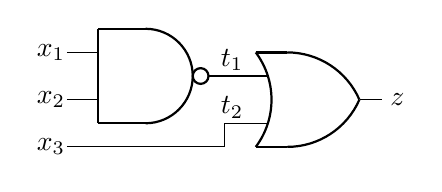
\begin{tikzpicture}[scale=0.20]
  %% NAND gate
   \draw [thick] (2,7.5) -- (5,7.5);
   \draw [thick] (2,1.5) -- (5,1.5);
   \draw [thick] (2,7.5) -- (2,1.5);
   \draw [thick] (5,1.5) arc [radius=3, start angle = -90, end angle = 90];
   \draw [thick] (8.5,4.5) circle [radius=0.5];
   %% OR gate
   \draw [thick] (12,6) -- (14,6);
   \draw [thick] (12,0) -- (14,0);
   \draw [thick] (12,6) arc [radius=5, start angle = 36.9, end angle = -36.9];
   \draw [thick] (14, 6) arc [radius=5, start angle = 90, end angle = 23.6];
   \draw [thick] (14, 0)  arc [radius=5, start angle = -90, end angle = -23.6];
   \draw (18.6,3) -- (20,3);
  %% Wire it up
  \draw (0,6) -- (2,6);
  \draw (0,3) -- (2,3);
  \draw (0,0) -- (10,0) -- (10,1.5) -- (12.8,1.5);
  \draw (9,4.5) -- (12.8,4.5);
  %% Put in labels
  \node at (-1,6) {$x_1$};
  \node at (-1,3) {$x_2$};
  \node at (-1,0) {$x_3$};
  \node at (10.5,5.5) {$t_1$};
  \node at (10.5,2.5) {$t_2$};
  \node at (21,3) {$z$};
\end{tikzpicture}
\end{center}
\renewcommand{\arraystretch}{1.1}
\begin{tabular}{lcc}
  \toprule
  \makebox[0.5in]{} & \makebox[1.75in]{Encode NAND gate} & \makebox[1.75in]{Encode OR gate} \\
  \midrule
  Formula
     & $\tnot_1 \leftrightarrow x_1 \land x_2$  
     & $z \leftrightarrow t_1 \lor t_2$  \\
  \midrule
  Clauses 
     &  $\begin{array}{l}
        t_1 \lor x_1 \\
       t_1 \lor x_2 \\
        \tnot_1 \lor \xnot_1 \lor \xnot_2\\
       \end{array}$
     &  $\begin{array}{l}
        \znot \lor t_1 \lor t_2 \\
        z \lor \tnot_1 \\
        z \lor \tnot_2 \\
       \end{array}$ \\
  \bottomrule
\end{tabular}

\medskip

    {\bf Tseitin Encoding}
    \begin{itemize}
    \item Introduce variables for intermediate values
    \item Linear complexity
    \end{itemize}


} %% FRAME

\frame{
  \frametitle{Proof Rules: Resolution}

\begin{itemize}
\item Robinson, 1965
\end{itemize}

\begin{center}
\begin{tikzpicture}
\onslide<+->{
\node at (2.5,0) {$\anot \lor b \lor \structure{x}$};
\node at (5,0) {$\structure{\xnot} \lor c \lor \dnot$};
\draw[thick] (1.5,-0.25) -- (6.2,-0.25);
\node at (3.75,-0.5) {$(\anot \lor b) \lor (c \lor \dnot)$};}
\onslide<+->{
\node at (1,1) {$(a \land \bnot) \rightarrow \structure{x}$};
\node at (6.5,1) {$\structure{x} \rightarrow (c \lor \dnot)$};}
\onslide<+->{
\node at (3.75,-1.5) {$(a \land \bnot) \rightarrow (c \lor \dnot)$};}
\end{tikzpicture}
\end{center}
\begin{itemize}
\item Generalization of implication
\item See  \hcref{https://en.wikipedia.org/wiki/Resolution\_(logic)}
\end{itemize}  


} %% FRAME

\frame{
  \frametitle{Resolution Principle Nuances}


\bigskip

{\bf OK To Have Repeated Literal}

\medskip

\begin{center}
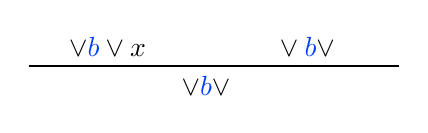
\begin{tikzpicture}
\node at (2.5,0) {$\anot \lor \textcolor{xblue}{b} \lor \structure{x}$};
\node at (5,0) {$\structure{\xnot} \lor \textcolor{xblue}{b} \lor \dnot$};
\draw[thick] (1.5,-0.25) -- (6.2,-0.25);
\node at (3.75,-0.5) {$\anot \lor \textcolor{xblue}{b} \lor \dnot$};
\end{tikzpicture}
\end{center}

\medskip

{\bf Not OK to Have Multiple Resolution Variables}

\medskip

\begin{center}
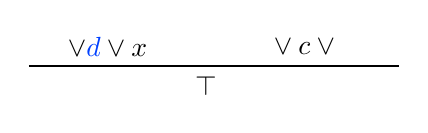
\begin{tikzpicture}
\node at (2.5,0) {$\anot \lor \textcolor{xblue}{d} \lor \structure{x}$};
\node at (5,0) {$\structure{\xnot} \lor c \lor \textcolor{xblue}{\dnot}$};
\draw[thick] (1.5,-0.25) -- (6.2,-0.25);
\node at (3.75,-0.5) {$\top$};
\end{tikzpicture}
\end{center}


} %% FRAME

\frame{
  \frametitle{Proof Rules: Subsumption}

  \bigskip
  
\begin{center}
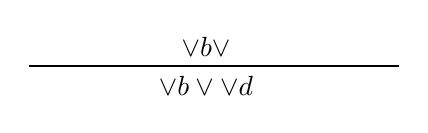
\begin{tikzpicture}
\node at (3.75,0) {$\anot \lor b \lor \cnot$};
\draw[thick] (1.5,-0.25) -- (6.2,-0.25);
\node at (3.75,-0.5) {$\anot \lor b \lor \cnot \lor \structure{d}$};
\end{tikzpicture}
\end{center}
\begin{itemize}
\item General Principle: $F \rightarrow F \lor d$
\end{itemize}  


} %% FRAME



\end{document}


\frame{
\frametitle{Clausal Proof}

\large

\bigskip

\begin{tikzpicture}
\node at (0,0) {
\begin{tabular}{cccc}
\rowcolor{structure}\textcolor{white}{Step} & \textcolor{white}{~~~Clause~~~} & 
\textcolor{white}{Antecedents} & \textcolor{white}{~~~Formula~~~}\\[3pt]
\rowcolor{structure!20!white} 1 & $\lnot v \lor w$ & & $v \rightarrow w$\\[3pt]
\rowcolor{structure!30!white}2 & $\lnot v \lor \lnot w$ & & $v \rightarrow \lnot w$\\[3pt]
\rowcolor{structure!20!white}3 & $v$ & & $v$\\[3pt]
\rowcolor{xblue!20!white}4 & $\lnot v$ & $1,2$ & $\lnot v$\\[3pt]
\rowcolor{xblue!30!white}5 & $\bot$ & $3,4$ & $v \land \lnot v$
\end{tabular}};

\draw [very thick,decorate,decoration={brace,amplitude=5pt},xshift=4pt,yshift=4pt] (4.25,1) -- (4.25,-0.75) node [black,midway,xshift=1cm, text width=1cm] {Input clauses};
\draw [very thick,decorate,decoration={brace,amplitude=5pt},xshift=4pt,yshift=4pt] (4.25,-0.85) -- (4.25,-1.85) node [black,midway,xshift=1cm, text width=1cm] {Derived clauses};

\end{tikzpicture}

\bigskip

\begin{itemize}
\item Prove conjunction of input clauses unsatisfiable
\item Add derived clauses
\begin{itemize}
\item Provides list of antecedent clauses that resolve to new clause
\end{itemize}
\item Finish with empty clause
\begin{itemize}
\item Proof is series of inferences leading to contradiction
\end{itemize}
\end{itemize}

}

\frame{
\frametitle{Extended Resolution}


{\bf Can introduce extension variables}
\begin{itemize}
\item Variable $e$ that has not yet occurred in proof
\item Must introduce defining clauses
\begin{itemize}
\item Clauses creating constraint of form $e \leftrightarrow F$
\item Boolean formula $F$ over input and earlier extension variables
\end{itemize}
\end{itemize}

\vspace{20pt}

{\bf Extension variable becomes shorthand for much larger formula}
  \begin{itemize}
  \item Through repeated application, can have exponentially smaller proof
  \end{itemize}




}

\frame{
\frametitle{Extended Resolution Example}


{\bf Example: Prove following set of constraints unsatisfiable}

\begin{center}
\begin{tabular}{ccc}
\rowcolor{structure}\textcolor{white}{~~~Constraint~~~} & \textcolor{white}{~~~Clauses~~~}\\[3pt]
\rowcolor{structure!20!white} $u \land v \rightarrow w$ & $\lnot u \lor \lnot v \lor w$\\
\rowcolor{structure!30!white}$u \land v \rightarrow \lnot w$ & $\lnot u \lor \lnot  v \lor \lnot w$\\
\rowcolor{structure!20!white}$u \land v$ & $u$\\
\rowcolor{structure!20!white} & $v$\\
\end{tabular}
\end{center}

%\vspace{-15pt}


\begin{itemize}\item Strategy: Introduce extension variable $e$ such that $e \leftrightarrow u \land v$
\end{itemize}

\begin{center}
\begin{tabular}{ccc}
\rowcolor{structure}\textcolor{white}{~~~Constraint~~~} & \textcolor{white}{~~~Clauses~~~}\\[3pt]
\rowcolor{xgreen!20!white} $u \land v  \rightarrow  e$ & $e \lor \lnot u \lor \lnot v$\\
\rowcolor{xgreen!30!white} $e \rightarrow  u$  & $\lnot e \lor u$ \\
\rowcolor{xgreen!20!white}  $e \rightarrow  v$ & $\lnot e \lor v$  \\
\end{tabular}
\end{center}

}


\frame{
\frametitle{ER Proof}

\parindent -10pt

\begin{tikzpicture}
\node at (0,0){
\begin{tabular}{cccc}
\rowcolor{structure}\textcolor{white}{Step} & \textcolor{white}{~~~Clause~~~} & 
\textcolor{white}{Antecedents} & \textcolor{white}{~~Formula~~} \\[3pt]
\rowcolor{structure!20!white}$1$ & $\lnot u \lor \lnot v \lor w$ & & $u \land v  \rightarrow  w$\\
\rowcolor{structure!30!white}$2$ & $\lnot u \lor \lnot v \lor \lnot w$ & & $u \land v  \rightarrow  \lnot w$\\
\rowcolor{structure!20!white}$3$ & $u$ & & $u$\\
\rowcolor{structure!30!white}$4$ & $v$ & & $v$\\
\rowcolor{xgreen!20!white}$5$ & $e \lor \lnot u \lor \lnot v$ & & $u \land v  \rightarrow  e$\\
\rowcolor{xgreen!30!white}$6$ & $\lnot e \lor u$ & & $e \rightarrow  u$ \\
\rowcolor{xgreen!20!white}$7$ & $\lnot e \lor v$ & & $e \rightarrow  v$ \\
\rowcolor{xblue!20!white}$8$ & $\lnot e \lor \lnot v \lor w$ &1, 6 & $e \land v  \rightarrow  w$ \\
\rowcolor{xblue!30!white}$9$ & $\lnot e \lor w$ &7, 8 & $e \rightarrow  w$ \\
\rowcolor{xblue!20!white}$10$ & $\lnot e \lor \lnot v \lor \lnot w$ & 2, 6 & $e \land v  \rightarrow  \lnot w$ \\
\rowcolor{xblue!30!white}$11$ & $\lnot e \lor \lnot w$ &7, 10 & $e \rightarrow  \lnot w$ \\
\rowcolor{xblue!20!white}$12$ & $e \lor \lnot v$ & 3, 5 & $v  \rightarrow  e$ \\
\rowcolor{xblue!30!white}$13$ & $e$ & 4, 12 & $e$ \\
\rowcolor{xblue!20!white}$14$ & $\lnot e$ &9, 11 & $\lnot e$ \\
\rowcolor{xblue!30!white}$15$ & $\bot$ & 13, 14 & $e \land \lnot e$ \\
\end{tabular}};

\draw [very thick,decorate,decoration={brace,amplitude=5pt},xshift=4pt,yshift=4pt] (4.5,3.2) -- (4.5,1.35) node [black,midway,xshift=1cm, text width=1cm] {Input clauses};
\draw [very thick,decorate,decoration={brace,amplitude=5pt},xshift=4pt,yshift=4pt] (4.5,1.25) -- (4.5,-.25) node [black,midway,xshift=1cm, text width=1cm] {Defining clauses};
\draw [very thick,decorate,decoration={brace,amplitude=5pt},xshift=4pt,yshift=4pt] (4.5,-0.35) -- (4.5,-4) node [black,midway,xshift=1cm, text width=1cm] {Derived clauses};

\only<2->{
\node[very thick, draw=structure, rectangle, minimum height=0.5cm, minimum width=2.5cm, rounded corners] (a) at (3,-0.75) {};
\node[very thick, draw=structure, rectangle, minimum height=0.5cm, minimum width=2.5cm, rounded corners] (b) at (3,-1.75) {};
\node[very thick, draw=structure, rectangle, minimum height=0.5cm, minimum width=2.5cm, rounded corners] (c) at (3,-2.65) {};

\node[text width=1.5cm] (d) at (6.5,-.7) {\structure{$u \land v$ replaced by $e$}};

\draw[thick, color=structure, -latex] (d) -- (a.east);
\draw[thick, color=structure, -latex] (d) -- (b.east);
\draw[thick, color=structure, -latex] (d) -- (c.east);}

\end{tikzpicture}

}



\frame{
\frametitle{Reduced, Ordered Binary Decision Diagrams (BDDs)}

\large

\begin{minipage}{.6\textwidth}
\begin{itemize}
\item Bryant, 1986
\end{itemize}
\medskip

{\bf Representation}
\begin{itemize}
\item Canonical representation of Boolean function
\item Compact for many useful cases
\end{itemize}
\medskip

{\bf Algorithms}
\begin{itemize}
\item ${\sf Apply}(f, g, op)$
\begin{itemize}
\item $op$ is Boolean operation\\(e.g., $\land$, $\lor$, $\oplus$)
\item BDD representation of $f~op~g$ 
\end{itemize}
\item ${\sf EQuant}(f, X)$
\begin{itemize}
\item $X$ set of variables
\item BDD representation of $\exists V f$
\end{itemize}
\end{itemize}
\end{minipage}
\hfill
\begin{minipage}{.38\textwidth}
%\includegraphics[width=\textwidth]{BDD.png}
\end{minipage}

}

\frame{
\frametitle{Apply Algorithm Recursion}

\bigskip

\begin{minipage}{.45\textwidth}
\centering
${\sf Apply} (u,v,\land)$\\[10pt]
\begin{tikzpicture}
\node[circle,draw,minimum size=0.75cm] (x) at (0,0) {$x$};
\node (u) at (-0.75,0) {$u$};
\node[circle,draw,minimum size=0.75cm] (l) at (-0.75,-1.3) {$~$};
\node (u1) at (-1.5,-1.3) {$u_0$};
\node[circle,draw,minimum size=0.75cm] (r) at (.75,-1.3) {$~$};
\node (u2) at (1.5,-1.3) {$u_1$};
\node[circle,minimum size=0.75cm] (ll) at (-1.3,-2.6) {$~$};
\node[circle,minimum size=0.75cm] (lr) at (-.2,-2.6) {$~$};
\node[circle,minimum size=0.75cm] (rl) at (.2,-2.6) {$~$};
\node[circle,minimum size=0.75cm] (rr) at (1.3,-2.6) {$~$};
\draw[thick, color=xgreen,densely dashed] (x) -- (l);
\draw[thick, color=structure] (x) -- (r);
\draw[thick, color=xgreen,densely dashed] (l) -- (ll);
\draw[thick, color=structure] (r) -- (rr);
\draw[thick, color=xgreen,densely dashed] (r) -- (rl);
\draw[thick, color=structure] (l) -- (lr);
\end{tikzpicture}

\bigskip

\begin{tikzpicture}
\node[circle,draw,minimum size=0.75cm] (x) at (0,0) {$x$};
\node (v) at (-0.75,0) {$v$};
\node[circle,draw,minimum size=0.75cm] (l) at (-0.75,-1.3) {$~$};
\node (v1) at (-1.5,-1.3) {$v_0$};
\node[circle,draw,minimum size=0.75cm] (r) at (.75,-1.3) {$~$};
\node (v2) at (1.5,-1.3) {$v_1$};
\node[circle,minimum size=0.75cm] (ll) at (-1.3,-2.6) {$~$};
\node[circle,minimum size=0.75cm] (lr) at (-.2,-2.6) {$~$};
\node[circle,minimum size=0.75cm] (rl) at (.2,-2.6) {$~$};
\node[circle,minimum size=0.75cm] (rr) at (1.3,-2.6) {$~$};
\draw[thick, color=xgreen,densely dashed] (x) -- (l);
\draw[thick, color=structure] (x) -- (r);
\draw[thick, color=xgreen,densely dashed] (l) -- (ll);
\draw[thick, color=structure] (r) -- (rr);
\draw[thick, color=xgreen,densely dashed] (r) -- (rl);
\draw[thick, color=structure] (l) -- (lr);
\end{tikzpicture}
\end{minipage}
\hfill
\begin{minipage}{.52\textwidth}
\centering
\pause
Recursion\\[5pt]

\begin{tikzpicture}
\node at (-2.3,-.2) {${\sf Apply} (u_1,v_1,\land)~\rightarrow~~~$};
\node[circle,draw,minimum size=0.75cm] (x) at (0,0) {~};
\node (u) at (0.75,0) {$w_1$};
\node[minimum size=0.75cm] (l) at (-0.75,-1.3) {$~$};
\node[minimum size=0.75cm] (r) at (.75,-1.3) {$~$};
\draw[thick, color=xgreen,densely dashed] (x) -- (l);
\draw[thick, color=structure] (x) -- (r);
\end{tikzpicture}
\begin{tikzpicture}
\node at (-2.3,-.2) {${\sf Apply} (u_0,v_0,\land)~\rightarrow~~~$};
\node[circle,draw,minimum size=0.75cm] (x) at (0,0) {~};
\node (u) at (0.75,0) {$w_0$};
\node[minimum size=0.75cm] (l) at (-0.75,-1.3) {$~$};
\node[minimum size=0.75cm] (r) at (.75,-1.3) {$~$};
\draw[thick, color=xgreen,densely dashed] (x) -- (l);
\draw[thick, color=structure] (x) -- (r);
\end{tikzpicture}

\vspace{-15pt}
\pause
Result\\[10pt]
\begin{tikzpicture}
\node[circle,draw,minimum size=0.75cm] (x) at (0,0) {$x$};
\node (w) at (-0.75,0) {$w$};
\node[circle,draw,minimum size=0.75cm] (l) at (-0.75,-1.3) {$~$};
\node (w1) at (-1.5,-1.3) {$w_0$};
\node[circle,draw,minimum size=0.75cm] (r) at (.75,-1.3) {$~$};
\node (w2) at (1.5,-1.3) {$w_1$};
\node[circle,minimum size=0.75cm] (ll) at (-1.3,-2.6) {$~$};
\node[circle,minimum size=0.75cm] (lr) at (-.2,-2.6) {$~$};
\node[circle,minimum size=0.75cm] (rl) at (.2,-2.6) {$~$};
\node[circle,minimum size=0.75cm] (rr) at (1.3,-2.6) {$~$};
\draw[thick, color=xgreen,densely dashed] (x) -- (l);
\draw[thick, color=structure] (x) -- (r);
\draw[thick, color=xgreen,densely dashed] (l) -- (ll);
\draw[thick, color=structure] (r) -- (rr);
\draw[thick, color=xgreen,densely dashed] (r) -- (rl);
\draw[thick, color=structure] (l) -- (lr);
\end{tikzpicture}

\end{minipage}

}

\frame{
\frametitle{Apply Algorithm Nuances}

{\bf Stop recursion when hit terminal case}
\begin{itemize}
\item $f \land 0	 \rightarrow	 0$ $\qquad\qquad$	$0 \land g 	 \rightarrow	 0$
\item $f \land 1	 \rightarrow	 f$ $\qquad\qquad$	$1 \land g 	 \rightarrow	 g$
\item $f \land f 	 \rightarrow	 f$
\end{itemize}
\smallskip

{\bf Special cases for recursion}
\begin{itemize}
\item $u$ and $v$ have different top-level variables
\item Recursion returns values with $w_1 = w_0$  
\end{itemize}  
\smallskip

{\bf Operation Cache contains previously computed results}
\begin{itemize}
\item $[u, v, \land] \rightarrow w$
\item Guarantees polynomial performance
\end{itemize}
\smallskip

{\bf Unique Table contains all generated nodes}
\begin{itemize}
\item $[x, u_1, u_0] \rightarrow u$
\item Guarantees canonical form of result
\end{itemize}




}


\frame{
\frametitle{Generating ER Proofs}

\begin{itemize}
\item Create extension variable for each node in BDD
\begin{itemize}
\item Notation: Same symbol for node and its extension variable
\end{itemize}
\end{itemize}

\begin{center}
\begin{tikzpicture}
\node[circle,draw,minimum size=0.75cm] (x) at (0,0) {$x$};
\node (u) at (-0.75,0) {$u$};
\node[circle,draw,minimum size=0.75cm] (l) at (-0.75,-1.3) {$~$};
\node (u1) at (-1.5,-1.3) {$u_0$};
\node[circle,draw,minimum size=0.75cm] (r) at (.75,-1.3) {$~$};
\node (u2) at (1.5,-1.3) {$u_1$};
\node[circle,minimum size=0.75cm] (ll) at (-1.3,-2.6) {$~$};
\node[circle,minimum size=0.75cm] (lr) at (-.2,-2.6) {$~$};
\node[circle,minimum size=0.75cm] (rl) at (.2,-2.6) {$~$};
\node[circle,minimum size=0.75cm] (rr) at (1.3,-2.6) {$~$};
\draw[thick, color=xgreen,densely dashed] (x) -- (l);
\draw[thick, color=structure] (x) -- (r);
\draw[thick, color=xgreen,densely dashed] (l) -- (ll);
\draw[thick, color=structure] (r) -- (rr);
\draw[thick, color=xgreen,densely dashed] (r) -- (rl);
\draw[thick, color=structure] (l) -- (lr);
\end{tikzpicture}
\end{center}

\vspace{-25pt}

\begin{itemize}
\item Defining clauses create constraint $u \leftrightarrow {\sf ITE}(x, u_1, u_0)$
\end{itemize}
\medskip

\centering

\begin{tabular}{ccc}
\rowcolor{structure}\textcolor{white}{Clause name} & \textcolor{white}{~~~Formula~~~} & 
\textcolor{white}{~~Clausal form~~} \\[3pt]
\rowcolor{xgreen!20!white} ${\sf HD}(u)$ & $x \rightarrow (u \rightarrow u_1)$ & $\lnot x \lor \lnot u \lor u_1$\\
\rowcolor{xgreen!30!white}${\sf LD}(u)$ & $\lnot x \rightarrow (u \rightarrow u_0)$ & $x \lor \lnot u \lor u_0$\\
\rowcolor{xgreen!20!white}${\sf HU}(u)$ & $x \rightarrow (u_1 \rightarrow u)$ & $\lnot x \lor \lnot u_1 \lor u$\\
\rowcolor{xgreen!30!white}${\sf LU}(u)$ & $\lnot x \rightarrow (u_0 \rightarrow u)$ & $x \lor \lnot u_0 \lor u$\\
\end{tabular}



}


\frame{
\frametitle{Proof-Generating Apply Operation}

{\bf Integrate Proof Generation into Apply Operation}
\begin{itemize}
\item When ${\sf Apply}(u, v,\land)$ returns $w$, also generate proof $u \land v \rightarrow w$
\item Store step number in operation cache
\item {\bf Key Idea:} Proof based on the underlying logic of the ${\sf Apply}$ algorithm
\end{itemize}

\bigskip
{\bf Proof Structure}
\begin{itemize}
\item Assume recursive calls generate proofs
\begin{itemize}
\item $u_1 \land v_1\rightarrow w_1$
\item $u_0 \land v_0\rightarrow w_0$
\end{itemize}
\item Combine with defining clauses for nodes $u$, $v$, and $w$
\end{itemize}

}

\frame{
\frametitle{Apply Proof Structure}

{\bf Defining Clauses}
\begin{center}
  \begin{tabular}{ccccc}
    \rowcolor{structure}\textcolor{white}{Clause} & \textcolor{white}{~~~Formula~~~} && \textcolor{white}{Clause} & \textcolor{white}{~~~Formula~~~} \\
\rowcolor{xgreen!20!white}    $\sf HD(u)$ & $x \rightarrow (u \rightarrow u_1)$ && $\sf LD(u)$ & $\lnot x \rightarrow (u \rightarrow u_0)$ \\
\rowcolor{xgreen!30!white}    $\sf HD(v)$ & $x \rightarrow (v \rightarrow v_1)$ && $\sf LD(v)$ & $\lnot x \rightarrow (v \rightarrow v_0)$ \\
\rowcolor{xgreen!20!white}    $\sf HU(w)$ & $x \rightarrow (w_1 \rightarrow w)$ && $\sf LU(w)$ & $\lnot x \rightarrow (w_0 \rightarrow w)$ \\
  \end{tabular}
\end{center}

{\bf Resolution Steps}
\begin{center}
\!\!\!\!\!\!\!\!\!
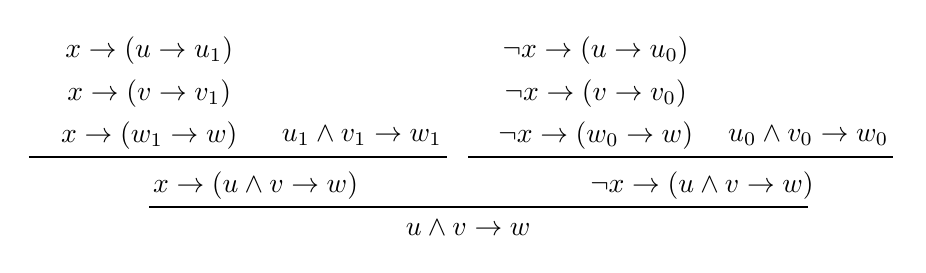
\begin{tikzpicture}[scale=0.9]

\node at (0,0) {$x \rightarrow (u \rightarrow u_1)$};
\node at (0,-0.6) {$x \rightarrow (v \rightarrow v_1)$};
\node at (0,-1.2) {$x \rightarrow (w_1 \rightarrow w)$};
\node at (3,-1.2) {$u_1 \land v_1 \rightarrow w_1$};

\draw[thick] (-1.7,-1.5) -- (4.2,-1.5);

\node at (1.5, -1.9) {$ x \rightarrow (u \land v \rightarrow w)$};

\node at (6.3,0) {$\lnot x \rightarrow (u \rightarrow u_0)$};
\node at (6.3,-0.6) {$\lnot x \rightarrow (v \rightarrow v_0)$};
\node at (6.3,-1.2) {$\lnot x \rightarrow (w_0 \rightarrow w)$};
\node at (9.3,-1.2) {$u_0 \land v_0 \rightarrow w_0$};

\draw[thick] (4.5,-1.5) -- (10.5,-1.5);

\node at (7.8, -1.9) {$\lnot x \rightarrow (u \land v \rightarrow w)$};

\draw[thick] (0,-2.2) -- (9.3,-2.2);


\node at (4.5, -2.5) {$u \land v \rightarrow w$};


\end{tikzpicture}
\end{center}
\!\!\!\!
{\bf Nuances}
\begin{itemize}
\item Many special cases when recursive arguments and results contain equivalences, 0s, and 1s.
\end{itemize}

}

\frame{
\frametitle{Quantification Operations}

{\bf Operation ${\sf EQuant}(f, X)$}
\begin{itemize}
\item Critical for obtaining good performance
\item Abstract away details of satisfying (partial) solutions
\end{itemize}

\bigskip

{\bf Proof Generation}
\begin{itemize}
\item Do not attempt to follow recursive structure of algorithm
\item Instead, follow with separate implication proof generation
\begin{itemize}
\item ${\sf EQuant}(u, X) \rightarrow w$
\item Generate proof $u \rightarrow w$
\item Algorithm similar to proof-generating Apply operation
\end{itemize}
\end{itemize}


}

\frame{
\frametitle{Overall Proof Task}

{\bf Input Variables}

\vspace{20pt}

{\bf Input Clauses}
\begin{itemize}
\item Set of input clauses $C_I$ over the input variables
\end{itemize}

\vspace{20pt}

{\bf Completion}
\begin{itemize}
\item Generate Proof $C_I \vdash \bot$
\end{itemize}

}


\frame{
\frametitle{Structure of Overall Proof}

{\bf Input Variables}
\begin{itemize}
\item Generate BDD variable for each input variable
\end{itemize}
{\bf Input Clauses}
\begin{itemize}
\item For each input clause $C \in C_I$, generate BDD representation $u$
\begin{itemize}
\item
 Using ${\sf Apply}$ with $\lor$ operation
\end{itemize}
\item Generate proof $C \vdash u$
\begin{itemize}
\item Sequence of resolution steps based on linear structure of BDD
\end{itemize}
\end{itemize}

{\bf Combine Top-Level BDDs}
\begin{itemize}
\item ${\sf Apply}(u, v, \land) \rightarrow w$
\begin{itemize}
\item Combine proofs $C_I \vdash u$, $C_I \vdash v$ and $u \land v \rightarrow w$ to get $C_I \vdash w$
\end{itemize}
\item ${\sf EQuant}(u, X) \rightarrow w$
\begin{itemize}
\item Combine proofs $C_I \vdash u$ and $u \rightarrow w$ to get $C_I \vdash w$
\end{itemize}
\end{itemize}
{\bf Completion}
\begin{itemize}
\item When ${\sf Apply}(u, v, \land) \rightarrow 0$ have proof $C_I \vdash \bot$
\end{itemize}

}


\frame{
\frametitle{Implementation}


{\bf Package}
\begin{itemize}
\item 2000 lines Python code (slow!)
\item BDD package + proof generator
\end{itemize}

\bigskip

{\bf Benchmark Generators}
\begin{itemize}
\item CNF file
\item File specifying ordering of variables
\item File specifying schedule:
\begin{itemize}
\item Defines sequence of conjunctions and quantifications
\end{itemize}
\end{itemize}

}


\frame{
\frametitle{Mutilated Chessboard Problem}

\begin{minipage}{.45\textwidth}
\centering
\begin{tikzpicture}[scale=0.65]
    
\foreach \x in {1, 2, 3, 4, 5} {
   \foreach \y in {1, 2, 3, 4, 5} {
     \ifodd\x
       \ifodd\y  % \x odd, \y odd
         \filldraw[whitefill] (\x, \y) -- (\x +1, \y) -- (\x +1, \y +1) -- (\x, \y +1) -- cycle;
         \filldraw[whitefill] (\x + 1, \y - 1) -- (\x + 2, \y - 1) -- (\x + 2, \y) -- (\x + 1, \y) -- cycle;
       \else  % \x odd, \y even
         \filldraw[grayfill] (\x, \y) -- (\x +1, \y) -- (\x +1, \y +1) -- (\x, \y +1) -- cycle;
         \filldraw[grayfill] (\x + 1, \y - 1) -- (\x + 2, \y - 1) -- (\x + 2, \y) -- (\x + 1, \y) -- cycle;
       \fi
     \else
       \ifodd\y  % \x even, \y odd
         \filldraw[grayfill] (\x, \y) -- (\x +1, \y) -- (\x +1, \y +1) -- (\x, \y +1) -- cycle;
         \filldraw[grayfill] (\x + 1, \y - 1) -- (\x + 2, \y - 1) -- (\x + 2, \y) -- (\x + 1, \y) -- cycle;
       \else  % \x even, \y even
         \filldraw[whitefill] (\x, \y) -- (\x +1, \y) -- (\x +1, \y +1) -- (\x, \y +1) -- cycle;
         \filldraw[whitefill] (\x + 1, \y - 1) -- (\x + 2, \y - 1) -- (\x + 2, \y) -- (\x + 1, \y) -- cycle;
       \fi
     \fi            
   }
}

\only<2->{
\draw [draw=black, fill=black, rounded corners=2pt] (2.1,0.1) rectangle (3.9,0.9);}

\only<3->{
\draw [draw=black, fill=black, rounded corners=2pt] (1.1,1.1) rectangle (2.9,1.9);
\draw [draw=black, fill=black, rounded corners=2pt] (1.1,2.1) rectangle (1.9,3.9);
\draw [draw=black, fill=black, rounded corners=2pt] (2.1,2.1) rectangle (2.9,3.9);
\draw [draw=black, fill=black, rounded corners=2pt] (1.1,4.1) rectangle (1.9,5.9);
\draw [draw=black, fill=black, rounded corners=2pt] (2.1,4.1) rectangle (3.9,4.9);
\draw [draw=black, fill=black, rounded corners=2pt] (2.1,5.1) rectangle (3.9,5.9);}

\only<4->{
\draw [draw=black, fill=black, rounded corners=2pt] (3.1,1.1) rectangle (3.9,2.9);
\draw [draw=black, fill=black, rounded corners=2pt] (4.1,1.1) rectangle (4.9,2.9);
\draw [draw=black, fill=black, rounded corners=2pt] (5.1,1.1) rectangle (5.9,2.9);
\draw [draw=black, fill=black, rounded corners=2pt] (6.1,0.1) rectangle (6.9,1.9);
\draw [draw=black, fill=black, rounded corners=2pt] (6.1,2.1) rectangle (6.9,3.9);
\draw [draw=black, fill=black, rounded corners=2pt] (4.1,0.1) rectangle (5.9,0.9);
\draw [draw=black, fill=black, rounded corners=2pt] (5.1,4.1) rectangle (6.9,4.9);
\draw [draw=black, fill=black, rounded corners=2pt] (3.1,3.1) rectangle (4.9,3.9);
\draw [draw=black, fill=black, rounded corners=2pt] (4.1,4.1) rectangle (4.9,5.9);

}

\end{tikzpicture}
\end{minipage}
\hfill
\begin{minipage}{.5\textwidth}
{\bf Definition}
\begin{itemize}
\item $N \times N$ chessboard with $2$ corners removed
\item Cover with tiles, each covering one square
\end{itemize}
\medskip
\pause\pause\pause
{\bf Solutions}
\begin{itemize}
\item None
\item More white squares than black\!\!\!\!
\item Each tile covers one white and one black square
\end{itemize}
\medskip
{\bf Proof}
\begin{itemize}
\item All resolution proofs of exponential size
\end{itemize}
\end{minipage}

}

%%%%%%%%%%%%%%%%%%%%%%%

\frame{
\frametitle{Encoding as SAT Problem}


\begin{minipage}{.22\textwidth}
\centering
\begin{tikzpicture}[scale=0.65]
\filldraw[grayfill] (0, 0) -- (1, 0) -- (1, 1) -- (0, 1) -- cycle;
\filldraw[whitefill] (-1, 0) -- (0, 0) -- (0, 1) -- (-1, 1) -- cycle;
\filldraw[whitefill] (1, 0) -- (2, 0) -- (2, 1) -- (1, 1) -- cycle;
\filldraw[whitefill] (0, -1) -- (1, -1) -- (1, 0) -- (0, 0) -- cycle;
\filldraw[whitefill] (0, 1) -- (1, 1) -- (1, 2) -- (0, 2) -- cycle;
\hdomino{0}{0}
\draw[very thick, color=xgreen] (0,0) -- (1,0);
\draw[very thick, color=structure] (1,0) -- (1,1);
\draw[very thick, color=xgreen] (1,1) -- (0,1);
\draw[very thick, color=xgreen] (0,1) -- (0,0);
\end{tikzpicture}
\end{minipage}
\begin{minipage}{.22\textwidth}
\centering
\begin{tikzpicture}[scale=0.65]
\filldraw[grayfill] (0, 0) -- (1, 0) -- (1, 1) -- (0, 1) -- cycle;
\filldraw[whitefill] (-1, 0) -- (0, 0) -- (0, 1) -- (-1, 1) -- cycle;
\filldraw[whitefill] (1, 0) -- (2, 0) -- (2, 1) -- (1, 1) -- cycle;
\filldraw[whitefill] (0, -1) -- (1, -1) -- (1, 0) -- (0, 0) -- cycle;
\filldraw[whitefill] (0, 1) -- (1, 1) -- (1, 2) -- (0, 2) -- cycle;
\vdomino{0}{-1}
\draw[very thick, color=structure] (0,0) -- (1,0);
\draw[very thick, color=xgreen] (1,0) -- (1,1);
\draw[very thick, color=xgreen] (1,1) -- (0,1);
\draw[very thick, color=xgreen] (0,1) -- (0,0);
\end{tikzpicture}
\end{minipage}
\begin{minipage}{.22\textwidth}
\centering
\begin{tikzpicture}[scale=0.65]
\filldraw[grayfill] (0, 0) -- (1, 0) -- (1, 1) -- (0, 1) -- cycle;
\filldraw[whitefill] (-1, 0) -- (0, 0) -- (0, 1) -- (-1, 1) -- cycle;
\filldraw[whitefill] (1, 0) -- (2, 0) -- (2, 1) -- (1, 1) -- cycle;
\filldraw[whitefill] (0, -1) -- (1, -1) -- (1, 0) -- (0, 0) -- cycle;
\filldraw[whitefill] (0, 1) -- (1, 1) -- (1, 2) -- (0, 2) -- cycle;
\hdomino{-1}{0}
\draw[very thick, color=xgreen] (0,0) -- (1,0);
\draw[very thick, color=xgreen] (1,0) -- (1,1);
\draw[very thick, color=xgreen] (1,1) -- (0,1);
\draw[very thick, color=structure] (0,1) -- (0,0);
\end{tikzpicture}
\end{minipage}
\begin{minipage}{.22\textwidth}
\centering
\begin{tikzpicture}[scale=0.65]
\filldraw[grayfill] (0, 0) -- (1, 0) -- (1, 1) -- (0, 1) -- cycle;
\filldraw[whitefill] (-1, 0) -- (0, 0) -- (0, 1) -- (-1, 1) -- cycle;
\filldraw[whitefill] (1, 0) -- (2, 0) -- (2, 1) -- (1, 1) -- cycle;
\filldraw[whitefill] (0, -1) -- (1, -1) -- (1, 0) -- (0, 0) -- cycle;
\filldraw[whitefill] (0, 1) -- (1, 1) -- (1, 2) -- (0, 2) -- cycle;
\vdomino{0}{0}
\draw[very thick, color=xgreen] (0,0) -- (1,0);
\draw[very thick, color=xgreen] (1,0) -- (1,1);
\draw[very thick, color=structure] (1,1) -- (0,1);
\draw[very thick, color=xgreen] (0,1) -- (0,0);
\end{tikzpicture}
\end{minipage}
\bigskip
\bigskip

Boolean variable for each boundary between two squares
\begin{itemize}
\item $(N -1) \cdot N - 2$ vertical boundaries	$x_{i,j}$
\item $(N -1) \cdot N - 2$ horizontal boundaries $y_{i,j}$
\end{itemize}

\medskip

Constraints
\begin{itemize}
\item For each square, exactly one of its boundary variables = 1
\end{itemize}

}

\frame{
\frametitle{Column Scanning}
{\bf Scanning}
\begin{itemize}
\item Add tiles for each column from left to right
\end{itemize}
\medskip
{\bf Observation}
\begin{itemize}
\item When placing tiles in column, only need to know which squares are already occupied
\end{itemize}

\medskip

\begin{minipage}{.45\textwidth}
\centering
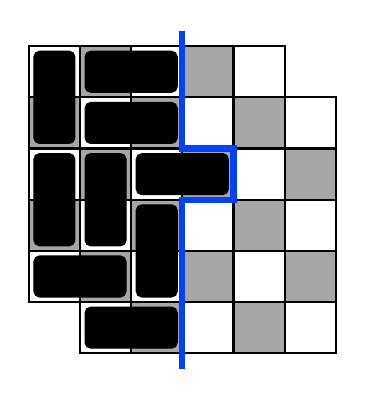
\begin{tikzpicture}[scale=0.65]
    
\foreach \x in {1, 2, 3, 4, 5} {
   \foreach \y in {1, 2, 3, 4, 5} {
     \ifodd\x
       \ifodd\y  % \x odd, \y odd
         \filldraw[whitefill] (\x, \y) -- (\x +1, \y) -- (\x +1, \y +1) -- (\x, \y +1) -- cycle;
         \filldraw[whitefill] (\x + 1, \y - 1) -- (\x + 2, \y - 1) -- (\x + 2, \y) -- (\x + 1, \y) -- cycle;
       \else  % \x odd, \y even
         \filldraw[grayfill] (\x, \y) -- (\x +1, \y) -- (\x +1, \y +1) -- (\x, \y +1) -- cycle;
         \filldraw[grayfill] (\x + 1, \y - 1) -- (\x + 2, \y - 1) -- (\x + 2, \y) -- (\x + 1, \y) -- cycle;
       \fi
     \else
       \ifodd\y  % \x even, \y odd
         \filldraw[grayfill] (\x, \y) -- (\x +1, \y) -- (\x +1, \y +1) -- (\x, \y +1) -- cycle;
         \filldraw[grayfill] (\x + 1, \y - 1) -- (\x + 2, \y - 1) -- (\x + 2, \y) -- (\x + 1, \y) -- cycle;
       \else  % \x even, \y even
         \filldraw[whitefill] (\x, \y) -- (\x +1, \y) -- (\x +1, \y +1) -- (\x, \y +1) -- cycle;
         \filldraw[whitefill] (\x + 1, \y - 1) -- (\x + 2, \y - 1) -- (\x + 2, \y) -- (\x + 1, \y) -- cycle;
       \fi
     \fi            
   }
}
\hdomino{1}{1}
\hdomino{2}{0} 
\vdomino{1}{2} 
\vdomino{2}{2} 
\vdomino{1}{4} 
\hdomino{2}{4} 
\hdomino{2}{5} 
\vdomino{3}{1} 
\hdomino{3}{3}

\draw [line width=0.8mm, xblue] (4,-0.3) -- (4,3) -- (5,3) -- (5,4) -- (4,4) -- (4,6.3);

\end{tikzpicture}
\end{minipage}
\hfill
\begin{minipage}{.45\textwidth}
\centering
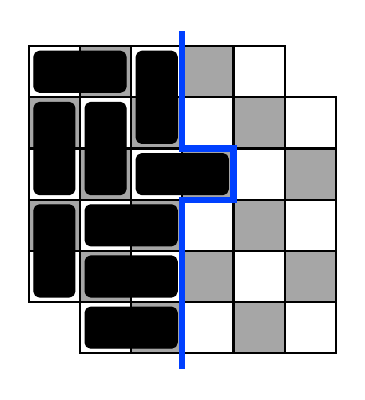
\begin{tikzpicture}[scale=0.65]
    
\foreach \x in {1, 2, 3, 4, 5} {
   \foreach \y in {1, 2, 3, 4, 5} {
     \ifodd\x
       \ifodd\y  % \x odd, \y odd
         \filldraw[whitefill] (\x, \y) -- (\x +1, \y) -- (\x +1, \y +1) -- (\x, \y +1) -- cycle;
         \filldraw[whitefill] (\x + 1, \y - 1) -- (\x + 2, \y - 1) -- (\x + 2, \y) -- (\x + 1, \y) -- cycle;
       \else  % \x odd, \y even
         \filldraw[grayfill] (\x, \y) -- (\x +1, \y) -- (\x +1, \y +1) -- (\x, \y +1) -- cycle;
         \filldraw[grayfill] (\x + 1, \y - 1) -- (\x + 2, \y - 1) -- (\x + 2, \y) -- (\x + 1, \y) -- cycle;
       \fi
     \else
       \ifodd\y  % \x even, \y odd
         \filldraw[grayfill] (\x, \y) -- (\x +1, \y) -- (\x +1, \y +1) -- (\x, \y +1) -- cycle;
         \filldraw[grayfill] (\x + 1, \y - 1) -- (\x + 2, \y - 1) -- (\x + 2, \y) -- (\x + 1, \y) -- cycle;
       \else  % \x even, \y even
         \filldraw[whitefill] (\x, \y) -- (\x +1, \y) -- (\x +1, \y +1) -- (\x, \y +1) -- cycle;
         \filldraw[whitefill] (\x + 1, \y - 1) -- (\x + 2, \y - 1) -- (\x + 2, \y) -- (\x + 1, \y) -- cycle;
       \fi
     \fi            
   }
}
\hdomino{2}{0} 
\vdomino{1}{1}
\hdomino{2}{1}
\hdomino{2}{2}
\vdomino{1}{3}
\vdomino{2}{3}
\hdomino{1}{5}
\vdomino{3}{4} 
\hdomino{3}{3}

\draw [line width=0.8mm, xblue] (4,-0.3) -- (4,3) -- (5,3) -- (5,4) -- (4,4) -- (4,6.3);

\end{tikzpicture}
\end{minipage}

}



\frame{
\frametitle{Abstraction Via Quantification}

\centering

\begin{minipage}{.45\textwidth}
\centering
\begin{tikzpicture}[scale=0.6]
    
\foreach \x in {1, 2, 3, 4, 5} {
   \foreach \y in {1, 2, 3, 4, 5} {
     \ifodd\x
       \ifodd\y  % \x odd, \y odd
         \filldraw[whitefill] (\x, \y) -- (\x +1, \y) -- (\x +1, \y +1) -- (\x, \y +1) -- cycle;
         \filldraw[whitefill] (\x + 1, \y - 1) -- (\x + 2, \y - 1) -- (\x + 2, \y) -- (\x + 1, \y) -- cycle;
       \else  % \x odd, \y even
         \filldraw[grayfill] (\x, \y) -- (\x +1, \y) -- (\x +1, \y +1) -- (\x, \y +1) -- cycle;
         \filldraw[grayfill] (\x + 1, \y - 1) -- (\x + 2, \y - 1) -- (\x + 2, \y) -- (\x + 1, \y) -- cycle;
       \fi
     \else
       \ifodd\y  % \x even, \y odd
         \filldraw[grayfill] (\x, \y) -- (\x +1, \y) -- (\x +1, \y +1) -- (\x, \y +1) -- cycle;
         \filldraw[grayfill] (\x + 1, \y - 1) -- (\x + 2, \y - 1) -- (\x + 2, \y) -- (\x + 1, \y) -- cycle;
       \else  % \x even, \y even
         \filldraw[whitefill] (\x, \y) -- (\x +1, \y) -- (\x +1, \y +1) -- (\x, \y +1) -- cycle;
         \filldraw[whitefill] (\x + 1, \y - 1) -- (\x + 2, \y - 1) -- (\x + 2, \y) -- (\x + 1, \y) -- cycle;
       \fi
     \fi            
   }
}

\hdomina{1}{1}
\hdomina{2}{0} 
\vdomina{1}{2} 
\vdomina{2}{2} 
\vdomina{1}{4} 
\hdomina{2}{4} 
\hdomina{2}{5} 
\vdomina{3}{1} 
\hdominah{3}{3} 

\node (a) at (7,2) {~};
\node (b) at (9,0) {~};
\draw[-latex, line width=2pt] (a) edge [bend left=40] (b);

\end{tikzpicture}
\end{minipage}
~~
\begin{minipage}{.45\textwidth}
\centering


\begin{tikzpicture}[scale=0.6]
    
\foreach \x in {1, 2, 3, 4, 5} {
   \foreach \y in {1, 2, 3, 4, 5} {
     \ifodd\x
       \ifodd\y  % \x odd, \y odd
         \filldraw[whitefill] (\x, \y) -- (\x +1, \y) -- (\x +1, \y +1) -- (\x, \y +1) -- cycle;
         \filldraw[whitefill] (\x + 1, \y - 1) -- (\x + 2, \y - 1) -- (\x + 2, \y) -- (\x + 1, \y) -- cycle;
       \else  % \x odd, \y even
         \filldraw[grayfill] (\x, \y) -- (\x +1, \y) -- (\x +1, \y +1) -- (\x, \y +1) -- cycle;
         \filldraw[grayfill] (\x + 1, \y - 1) -- (\x + 2, \y - 1) -- (\x + 2, \y) -- (\x + 1, \y) -- cycle;
       \fi
     \else
       \ifodd\y  % \x even, \y odd
         \filldraw[grayfill] (\x, \y) -- (\x +1, \y) -- (\x +1, \y +1) -- (\x, \y +1) -- cycle;
         \filldraw[grayfill] (\x + 1, \y - 1) -- (\x + 2, \y - 1) -- (\x + 2, \y) -- (\x + 1, \y) -- cycle;
       \else  % \x even, \y even
         \filldraw[whitefill] (\x, \y) -- (\x +1, \y) -- (\x +1, \y +1) -- (\x, \y +1) -- cycle;
         \filldraw[whitefill] (\x + 1, \y - 1) -- (\x + 2, \y - 1) -- (\x + 2, \y) -- (\x + 1, \y) -- cycle;
       \fi
     \fi            
   }
}

\hdomina{2}{0} 
\vdomina{1}{1}
\hdomina{2}{1}
\hdomina{2}{2}
\vdomina{1}{3}
\vdomina{2}{3}
\hdomina{1}{5}
\vdomina{3}{4} 
\hdominah{3}{3}

\node (a) at (1,2) {~};
\node (b) at (-1,0) {~};
\draw[-latex, line width=2pt] (a) edge [bend right=40] (b);

\end{tikzpicture}
\end{minipage}

\parindent -20pt
\begin{minipage}{.33\textwidth}
{\bf Scanning ``State''}
\begin{itemize}
\item $X_j$ = Value of vertical variables to right of column $j$.
\end{itemize}
\end{minipage}
~~
\begin{minipage}{.6\textwidth}
\begin{tikzpicture}[scale=0.6]
    
\foreach \x in {1, 2, 3, 4, 5} {
   \foreach \y in {1, 2, 3, 4, 5} {
     \ifodd\x
       \ifodd\y  % \x odd, \y odd
         \filldraw[whitefill] (\x, \y) -- (\x +1, \y) -- (\x +1, \y +1) -- (\x, \y +1) -- cycle;
         \filldraw[whitefill] (\x + 1, \y - 1) -- (\x + 2, \y - 1) -- (\x + 2, \y) -- (\x + 1, \y) -- cycle;
       \else  % \x odd, \y even
         \filldraw[grayfill] (\x, \y) -- (\x +1, \y) -- (\x +1, \y +1) -- (\x, \y +1) -- cycle;
         \filldraw[grayfill] (\x + 1, \y - 1) -- (\x + 2, \y - 1) -- (\x + 2, \y) -- (\x + 1, \y) -- cycle;
       \fi
     \else
       \ifodd\y  % \x even, \y odd
         \filldraw[grayfill] (\x, \y) -- (\x +1, \y) -- (\x +1, \y +1) -- (\x, \y +1) -- cycle;
         \filldraw[grayfill] (\x + 1, \y - 1) -- (\x + 2, \y - 1) -- (\x + 2, \y) -- (\x + 1, \y) -- cycle;
       \else  % \x even, \y even
         \filldraw[whitefill] (\x, \y) -- (\x +1, \y) -- (\x +1, \y +1) -- (\x, \y +1) -- cycle;
         \filldraw[whitefill] (\x + 1, \y - 1) -- (\x + 2, \y - 1) -- (\x + 2, \y) -- (\x + 1, \y) -- cycle;
       \fi
     \fi            
   }
}

\hdomino{3}{3}


\draw[very thick, color=xgreen] (4,0) -- (4,3);
\draw[very thick, color=structure] (4,3) -- (4,4);
\draw[very thick, color=xgreen] (4,4) -- (4,6);

\end{tikzpicture}
\end{minipage}

}


\frame{
\frametitle{Symbolic Computation of State Sets}

\parindent -10pt

\begin{minipage}{.30\textwidth}
\centering
State at column $j$-$1$\\
$\sigma_{j-1}(X_{j-1})$\\[5pt]
\begin{tikzpicture}[scale=0.6]
    
\foreach \x in {1, 2, 3, 4, 5} {
   \foreach \y in {1, 2, 3, 4, 5} {
     \ifodd\x
       \ifodd\y  % \x odd, \y odd
         \filldraw[whitefill] (\x, \y) -- (\x +1, \y) -- (\x +1, \y +1) -- (\x, \y +1) -- cycle;
         \filldraw[whitefill] (\x + 1, \y - 1) -- (\x + 2, \y - 1) -- (\x + 2, \y) -- (\x + 1, \y) -- cycle;
       \else  % \x odd, \y even
         \filldraw[grayfill] (\x, \y) -- (\x +1, \y) -- (\x +1, \y +1) -- (\x, \y +1) -- cycle;
         \filldraw[grayfill] (\x + 1, \y - 1) -- (\x + 2, \y - 1) -- (\x + 2, \y) -- (\x + 1, \y) -- cycle;
       \fi
     \else
       \ifodd\y  % \x even, \y odd
         \filldraw[grayfill] (\x, \y) -- (\x +1, \y) -- (\x +1, \y +1) -- (\x, \y +1) -- cycle;
         \filldraw[grayfill] (\x + 1, \y - 1) -- (\x + 2, \y - 1) -- (\x + 2, \y) -- (\x + 1, \y) -- cycle;
       \else  % \x even, \y even
         \filldraw[whitefill] (\x, \y) -- (\x +1, \y) -- (\x +1, \y +1) -- (\x, \y +1) -- cycle;
         \filldraw[whitefill] (\x + 1, \y - 1) -- (\x + 2, \y - 1) -- (\x + 2, \y) -- (\x + 1, \y) -- cycle;
       \fi
     \fi            
   }
}

\hdomino{3}{3}

\draw[very thick, color=xgreen] (4,0) -- (4,3);
\draw[very thick, color=structure] (4,3) -- (4,4);
\draw[very thick, color=xgreen] (4,4) -- (4,6);

\end{tikzpicture}
\end{minipage}
~~~
\begin{minipage}{.30\textwidth}
\centering
Column $j$ transition\\
$T_j(X_{j-1},Y_j,X_j)$\\[5pt]
\begin{tikzpicture}[scale=0.6]
    
\foreach \x in {1, 2, 3, 4, 5} {
   \foreach \y in {1, 2, 3, 4, 5} {
     \ifodd\x
       \ifodd\y  % \x odd, \y odd
         \filldraw[whitefill] (\x, \y) -- (\x +1, \y) -- (\x +1, \y +1) -- (\x, \y +1) -- cycle;
         \filldraw[whitefill] (\x + 1, \y - 1) -- (\x + 2, \y - 1) -- (\x + 2, \y) -- (\x + 1, \y) -- cycle;
       \else  % \x odd, \y even
         \filldraw[grayfill] (\x, \y) -- (\x +1, \y) -- (\x +1, \y +1) -- (\x, \y +1) -- cycle;
         \filldraw[grayfill] (\x + 1, \y - 1) -- (\x + 2, \y - 1) -- (\x + 2, \y) -- (\x + 1, \y) -- cycle;
       \fi
     \else
       \ifodd\y  % \x even, \y odd
         \filldraw[grayfill] (\x, \y) -- (\x +1, \y) -- (\x +1, \y +1) -- (\x, \y +1) -- cycle;
         \filldraw[grayfill] (\x + 1, \y - 1) -- (\x + 2, \y - 1) -- (\x + 2, \y) -- (\x + 1, \y) -- cycle;
       \else  % \x even, \y even
         \filldraw[whitefill] (\x, \y) -- (\x +1, \y) -- (\x +1, \y +1) -- (\x, \y +1) -- cycle;
         \filldraw[whitefill] (\x + 1, \y - 1) -- (\x + 2, \y - 1) -- (\x + 2, \y) -- (\x + 1, \y) -- cycle;
       \fi
     \fi            
   }
}

\vdomina{4}{0}
\hdomino{3}{3}
\hdomino{4}{2}
\hdomino{4}{4}
\hdomino{4}{5}

\draw[very thick, color=xgreen] (5,0) -- (5,2);
\draw[very thick, color=structure] (5,2) -- (5,3);
\draw[very thick, color=xgreen] (5,3) -- (5,4);
\draw[very thick, color=structure] (5,4) -- (5,6);


\draw[very thick, color=xgreen] (4,0) -- (4,3);
\draw[very thick, color=structure] (4,3) -- (4,4);
\draw[very thick, color=xgreen] (4,4) -- (4,6);

\draw[very thick, color=xgreen] (4,3) -- (5,3);
\draw[very thick, color=xgreen] (4,4) -- (5,4);
\draw[very thick, color=xgreen] (4,5) -- (5,5);
\draw[very thick, color=xgreen] (4,6) -- (5,6);


\end{tikzpicture}
\end{minipage}
~~~
\begin{minipage}{.30\textwidth}
\centering
State at column $j$\\
$\sigma_{j}(X_{j})$\\[5pt]
\begin{tikzpicture}[scale=0.6]
    
\foreach \x in {1, 2, 3, 4, 5} {
   \foreach \y in {1, 2, 3, 4, 5} {
     \ifodd\x
       \ifodd\y  % \x odd, \y odd
         \filldraw[whitefill] (\x, \y) -- (\x +1, \y) -- (\x +1, \y +1) -- (\x, \y +1) -- cycle;
         \filldraw[whitefill] (\x + 1, \y - 1) -- (\x + 2, \y - 1) -- (\x + 2, \y) -- (\x + 1, \y) -- cycle;
       \else  % \x odd, \y even
         \filldraw[grayfill] (\x, \y) -- (\x +1, \y) -- (\x +1, \y +1) -- (\x, \y +1) -- cycle;
         \filldraw[grayfill] (\x + 1, \y - 1) -- (\x + 2, \y - 1) -- (\x + 2, \y) -- (\x + 1, \y) -- cycle;
       \fi
     \else
       \ifodd\y  % \x even, \y odd
         \filldraw[grayfill] (\x, \y) -- (\x +1, \y) -- (\x +1, \y +1) -- (\x, \y +1) -- cycle;
         \filldraw[grayfill] (\x + 1, \y - 1) -- (\x + 2, \y - 1) -- (\x + 2, \y) -- (\x + 1, \y) -- cycle;
       \else  % \x even, \y even
         \filldraw[whitefill] (\x, \y) -- (\x +1, \y) -- (\x +1, \y +1) -- (\x, \y +1) -- cycle;
         \filldraw[whitefill] (\x + 1, \y - 1) -- (\x + 2, \y - 1) -- (\x + 2, \y) -- (\x + 1, \y) -- cycle;
       \fi
     \fi            
   }
}

\hdomino{4}{2}
\hdomino{4}{4}
\hdomino{4}{5}

\draw[very thick, color=xgreen] (5,0) -- (5,2);
\draw[very thick, color=structure] (5,2) -- (5,3);
\draw[very thick, color=xgreen] (5,3) -- (5,4);
\draw[very thick, color=structure] (5,4) -- (5,6);


\end{tikzpicture}
\end{minipage}

\parindent 0pt

{\Large
$$ \sigma_j(X_j) = \exists X_{j-1} [ \sigma_{j-1} (X_{j-1}) \land \exists Y_j T_j (X_{j-1},Y_j,X_j)]$$
}

\vspace{-10pt}

\begin{itemize}
\item Does not redefine underlying problem
\item Way to order conjunctions and quantifications
\end{itemize}

}


\frame{
\frametitle{Representing State Sets}

\begin{minipage}{.49\textwidth}
\!\!\!\!\!\!\!
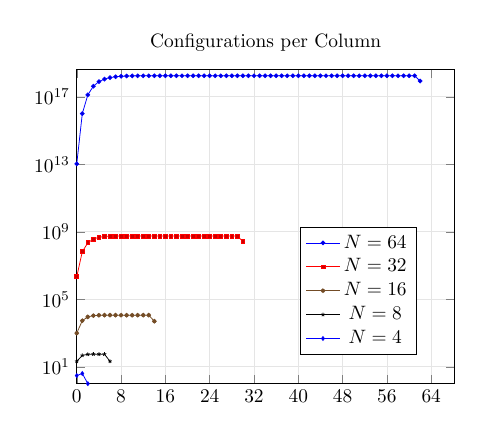
\begin{tikzpicture}[scale=0.7]
  \begin{axis}[mark options={scale=0.5},title=Configurations per Column, grid=both, grid style={black!10}, xtick={0, 8, 16, 24, 32, 40, 48, 56, 64}, xmin =0, ymode=log, ymin=1, ymax = 4000000000000000000, legend style={at={(0.9,0.5)}}]  

\addplot coordinates {(0, 10610209857723) (1, 10148305864982900) (2, 130530268521734000) (3, 428215143880080000) (4, 797698648315872000) (5, 1129492438558750000) (6, 1380255924944720000) (7, 1550072339944280000) (8, 1655638066432280000) (9, 1716362509304330000) (10, 1748750476658400000) (11, 1764768509224510000) (12, 1772109017099870000) (13, 1775222178953180000) (14, 1776442030128600000) (15, 1776882701365720000) (16, 1777029083506770000) (17, 1777073654992020000) (18, 1777086048255050000) (19, 1777089180996540000) (20, 1777089897051740000) (21, 1777090044098790000) (22, 1777090071018160000) (23, 1777090075369350000) (24, 1777090075982940000) (25, 1777090076057280000) (26, 1777090076064860000) (27, 1777090076065490000) (28, 1777090076065540000) (29, 1777090076065540000) (30, 1777090076065540000) (31, 1777090076065540000) (32, 1777090076065540000) (33, 1777090076065540000) (34, 1777090076065540000) (35, 1777090076065540000) (36, 1777090076065540000) (37, 1777090076065540000) (38, 1777090076065540000) (39, 1777090076065540000) (40, 1777090076065540000) (41, 1777090076065540000) (42, 1777090076065540000) (43, 1777090076065540000) (44, 1777090076065540000) (45, 1777090076065540000) (46, 1777090076065540000) (47, 1777090076065540000) (48, 1777090076065540000) (49, 1777090076065540000) (50, 1777090076065540000) (51, 1777090076065540000) (52, 1777090076065540000) (53, 1777090076065540000) (54, 1777090076065540000) (55, 1777090076065540000) (56, 1777090076065540000) (57, 1777090076065540000) (58, 1777090076065540000) (59, 1777090076065540000) (60, 1777090076065540000) (61, 1777090076065540000) (62, 860778005594247000)};

\addplot coordinates {(0, 2178309) (1, 66484244) (2, 222324436) (3, 373128151) (4, 473198136) (5, 527156117) (6, 551838565) (7, 561450672) (8, 564615152) (9, 565485384) (10, 565681800) (11, 565717264) (12, 565722192) (13, 565722687) (14, 565722719) (15, 565722720) (16, 565722720) (17, 565722720) (18, 565722720) (19, 565722720) (20, 565722720) (21, 565722720) (22, 565722720) (23, 565722720) (24, 565722720) (25, 565722720) (26, 565722720) (27, 565722720) (28, 565722720) (29, 565722720) (30, 265182525)};

\addplot coordinates {(0, 987) (1, 5373) (2, 9061) (3, 10760) (4, 11304) (5, 11423) (6, 11439) (7, 11440) (8, 11440) (9, 11440) (10, 11440) (11, 11440) (12, 11440) (13, 11440) (14, 5005)};
 
 \addplot coordinates {(0, 21) (1, 47) (2, 55) (3, 56) (4, 56) (5, 56) (6, 21)};
 
 \addplot coordinates {(0,3) (1,4) (2,1)};
         
          \legend{$N=64$, $N=32$, $N=16$, $N=8$, $N=4$}

\end{axis}                   
\end{tikzpicture}
\end{minipage}
\begin{minipage}{.49\textwidth}
\!\!\!\!\!\!\!
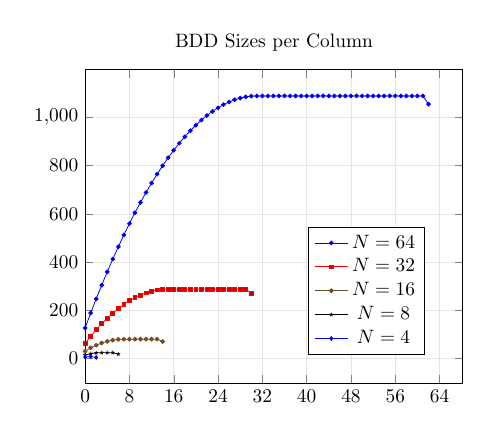
\begin{tikzpicture}[scale=0.7]
          \begin{axis}[mark options={scale=0.5},title=BDD Sizes per Column, grid=both, grid style={black!10}, xtick={0, 8, 16, 24, 32, 40, 48, 56, 64}, xmin = 0, legend style={at={(0.9,0.5)}}]  

\addplot coordinates {(0, 127) (1, 189) (2, 248) (3, 305) (4, 360) (5, 413) (6, 464) (7, 513) (8, 560) (9, 605) (10, 648) (11, 689) (12, 728) (13, 765) (14, 800) (15, 833) (16, 864) (17, 893) (18, 920) (19, 945) (20, 968) (21, 989) (22, 1008) (23, 1025) (24, 1040) (25, 1053) (26, 1064) (27, 1073) (28, 1080) (29, 1085) (30, 1088) (31, 1089) (32, 1089) (33, 1089) (34, 1089) (35, 1089) (36, 1089) (37, 1089) (38, 1089) (39, 1089) (40, 1089) (41, 1089) (42, 1089) (43, 1089) (44, 1089) (45, 1089) (46, 1089) (47, 1089) (48, 1089) (49, 1089) (50, 1089) (51, 1089) (52, 1089) (53, 1089) (54, 1089) (55, 1089) (56, 1089) (57, 1089) (58, 1089) (59, 1089) (60, 1089) (61, 1089) (62, 1055)};

\addplot coordinates {(0, 63) (1, 93) (2, 120) (3, 145) (4, 168) (5, 189) (6, 208) (7, 225) (8, 240) (9, 253) (10, 264) (11, 273) (12, 280) (13, 285) (14, 288) (15, 289) (16, 289) (17, 289) (18, 289) (19, 289) (20, 289) (21, 289) (22, 289) (23, 289) (24, 289) (25, 289) (26, 289) (27, 289) (28, 289) (29, 289) (30, 271)};

\addplot coordinates {(0, 31) (1, 45) (2, 56) (3, 65) (4, 72) (5, 77) (6, 80) (7, 81) (8, 81) (9, 81) (10, 81) (11, 81) (12, 81) (13, 81) (14, 71)};
 
 \addplot coordinates {(0, 15) (1, 21) (2, 24) (3, 25) (4, 25) (5, 25) (6, 19)};
 
 \addplot coordinates {(0, 7) (1, 9) (2, 5)};
         
          \legend{$N=64$, $N=32$, $N=16$, $N=8$, $N=4$}

\end{axis}                   
\end{tikzpicture}
\end{minipage}

\bigskip

\begin{itemize}
\item Number of configurations $\sim 2^N$
\item BDD representation $\sim N^2$
\item Reaches fixed point after column $N / 2$
\end{itemize}


}


\frame{
\frametitle{Chess Proof Complexity}


~~~~~~~~~~~~~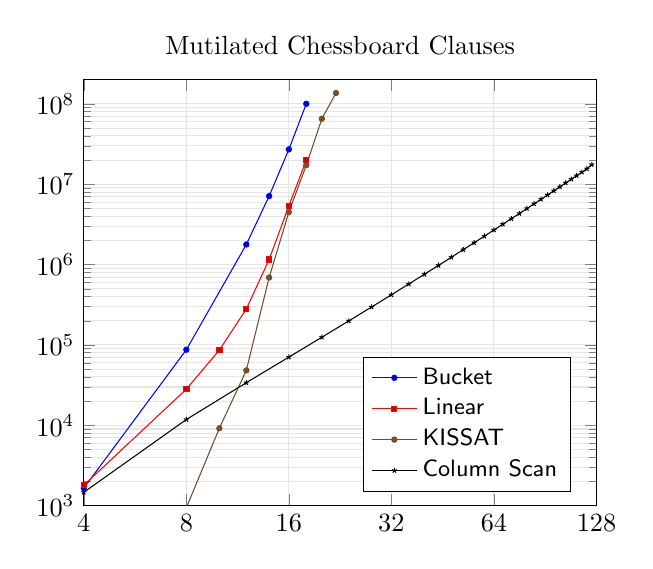
\begin{tikzpicture}[scale = .95]
          \begin{axis}[mark options={scale=0.5},grid=both, grid style={black!10}, xmode=log, ymode=log, legend style={at={(0.95,0.35)}}, legend cell align={left},
                              xtick={4,8,16,32,64,128}, xticklabels={$4$,$8$,$16$,$32$,$64$,$128$},xmin=4,xmax=128,ymin=1000,ymax=200000000, title={Mutilated Chessboard Clauses}]
\addplot coordinates { (4, 1653) (8, 87247) (12, 1781599) (14, 7122088) (16, 27197901) (18, 100406354)};
\addplot coordinates { (4, 1795) (8, 28180) (10, 86368) (12, 280104) (14, 1157658) (16, 5387291) (18, 19931662)};
\addplot coordinates { (4, 58) (6, 204) (8, 942) (10, 9180) (12, 48296) (14, 691551) (16, 4503635) (18, 17281161) (20, 65376268) (22, 136883320)};
\addplot coordinates { (4, 1466) (8, 11805) (12, 33919) (16, 70638) (20, 124849) (24, 199432) (28, 297267) (32, 421234) (36, 574213) (40, 759084) (44, 978727) (48, 1236022) (52, 1533849) (56, 1875088) (60, 2262619) (64, 2699322) (68, 3188077) (72, 3731764) (76, 4333263) (80, 4995454) (84, 5721217) (88, 6513432) (92, 7374979) (96, 8308738) (100, 9317589) (104, 10404412) (108, 11572087) (112, 12823494) (116, 14161513) (120, 15589024)(124,17581470)};%%           \addplot coordinates {(4, 1893) (8, 15411) (12, 43601) (16, 89264) (20, 155289) (24, 244576) (28, 359995) (32, 504436) (36, 680827) (40, 891930)
%%                                              (44, 1140685) (48, 1429972) (52, 1762671) (56, 2141662) (60, 2569825) (64, 3050040) (68, 3585187) (72, 4178146)
%%                                              (76, 4831797) (80, 5549020) (84, 6332695) (88, 7185702) (92, 8110921) (96, 9111232) (100, 10189515)};
%%          \addplot  coordinates {(4, 2643) (8, 34187) (10, 88063) (12, 378127) (14, 1074904) (16, 5520271) (18, 23086597)};
%%          \addplot [mark=triangle*] coordinates {(4, 2570) (8, 191586) (10, 1147177) (12, 6188911) (14, 31153105) (16, 149853103)};
            \legend{\small \textsf{Bucket}, \small \textsf{Linear}, \small \textsf{KISSAT}, \small \textsf{Column Scan}}
          \end{axis}
\end{tikzpicture}



\begin{itemize}
\item Problem size $\sim N^2$
\item Proof size $\sim N^{2.69}$
\end{itemize}

}


\frame{
\frametitle{Observations}

{\bf Key Insight}
\begin{itemize}
\item Sinz, Biere, and Jussila 
\item Capture underlying logic of BDD algorithms as ER proofs
\end{itemize}

\bigskip

{\bf Our Contributions}
\begin{itemize}
\item Integrate proof generation with Apply operations
\item Handle arbitrary existential quantification
\item Demonstrate on variety of benchmarks
\begin{itemize}
\item Mutilated chessboard
\item Pigeonhole principle
\item Parity formulas
\item Urquhart formulas
\end{itemize}
\end{itemize}



}

\frame{
\frametitle{Further Work}

{\bf Higher Performance Implementation}
\begin{itemize}
\item Integrate into existing BDD package
\end{itemize}
\medskip
{\bf More Automation}
\begin{itemize}
\item Variable Ordering
\item Conjunction and quantification scheduling
\end{itemize}
\medskip
{\bf Apply to Other Problems}
\begin{itemize}
\item QBF
\item Model checking
\item Model counting
\end{itemize}


}

\end{document}

%%% Local Variables:
%%% mode: latex
%%% TeX-master: t
%%% End:
